\documentclass[12pt]{report}
\usepackage[hmargin={1.5cm,1.5cm},vmargin={1.5cm,1.5cm}]{geometry}
\usepackage[brazil]{babel}
\usepackage[utf8]{inputenc}
\usepackage{amsbsy}
\usepackage{amscd,amsfonts,amsmath,amssymb,amstext,amsthm}
\usepackage{pgf,tikz}
\usepackage{mathrsfs}
\usetikzlibrary{arrows}
%\usepackage[brazil]{babel}
\usepackage{epsfig}
\usepackage{fancybox}
\usepackage{setspace}
\usepackage{latexsym}
\usepackage{niceframe}
\usepackage{srcltx}
\usepackage{enumerate}
\usepackage{multicol}
\usepackage{hyperref}
\usepackage{gensymb}
\usepackage{scrextend}
\usepackage{graphicx}
\usepackage{enumitem}
\usepackage{xcolor}
\hypersetup{
    colorlinks=false,
    linkcolor=blue,
    linkbordercolor=blue,
    filecolor=magenta,      
    urlcolor=cyan,
}
\newcommand{\ex}[1]{\hypertarget{ex#1}{\noindent\hyperlink{gab#1}{\textcolor{red}{\textbf{Ex.#1}}}}}
\newcommand{\gab}[1]{\hypertarget{gab#1}{\noindent\hyperlink{ex#1}{\textcolor{red}{\textbf{Ex.#1}}}}}
\newenvironment{Figure}
  {\par\medskip\noindent\minipage{\linewidth}}
  {\endminipage\par\medskip}

\renewcommand{\baselinestretch}{1.2}          % DISTÂNCIA ENTRE LINHAS
\begin{document}
\onehalfspacing
\begin{center}
\font\border=umrandb
\generalframe{\border\char'165}{\border\char'151}{\border\char'164}
             {\border\char'150}                  {\border\char'150}
             {\border\char'166}{\border\char'151}{\border\char'167}
             {
\begin{minipage}[c]{15cm}{
\vspace{0.3cm}
\begin{center}

\includegraphics[scale=0.5]{figures/lima_castro.png} \hspace{0.3cm} {\bf Escola Estadual Professor Lima Castro}\\
{\small \textbf{Disciplina}: Matemática} \hspace{0.1 cm}\\ \small{\textbf{Prof}.: Fernando Jorge}\\
\small{$1^{a}$ Lista de Exercícios - Data}\\
\vspace{0.3 cm}
\small{Funções do Primeiro Grau}\\
\end{center}}
\end{minipage}}
\end{center}
\begin{multicols}{2}
[
\begin{center}
\section*{Exercícios Gerais}
\end{center}
]
\changefontsizes[9pt]{9pt}

\ex{1} Dada a função $f:A \rightarrow B$, com $A={-1,0,1}$ e $B={-3,2,4}$, definida por $f(x) = 5x^2 - 3$, determine a $Im_{(f)}$ e construa um diagrama de flechas que representa essa função.

\ex{2} Sejam os conjuntos $A=\{1,3,5,7,9,11,13\}$ e $B=\{0,2,4,6,8,10,12\}$. Data a função $f:A \rightarrow B$, definida por $f(x) = x - 1$, determine o $D_{(f)}$, o $CD_{(f)}$, a $Im_{(f)}$ e construa o diagrama de flechas que representa ess função.

\ex{3} Considere uma função $f:A \rightarrow B$ em que:
\begin{enumerate}[label=\alph*)]
	\item $D_{(f)} = \{3,9,12\}$
	\item $CD_{(f)} = \{-3,-1,0,5,10,15\}$
	\item $Im_{(f)} = \{-3,0,10\}$
	\item $f(3) = -3$
	\item $f(9) = 0$
	\item $f(12) = 10$
\end{enumerate}
De acordo com as informações, represente a função \textit{f} por meio de um diagrama de flechas.

\ex{4} Seja a função $f:A \rightarrow B$ dada pela lei de formação $f(x)=3+x$. Determine o elemento de \textit{A} cuja imagem é $2$.

\ex{5} Sendo \textit{h} uma função de $A=\{x \in \mathbb{Z} \setminus 1 \leqslant x \leqslant 5\}$ em $\mathbb{Z}$, determine $Im_{(h)}$ quando \textit{h} for definida por:
\begin{enumerate}[label=\alph*)]
	\item $h(x) = \frac{120}{x} $
	\item $h(x) = \frac{120}{x+1} $
	\item $h(x) = \frac{120}{x}+1 $
	\item $h(x) = \frac{120}{x}-1 $
\end{enumerate}
	

\ex{6} Um motorista de táxi cobra, em cada corrida, o valor fixo de R\$ $3,20$ mais R\$ $0,80$ por quilômetro rodado.
\begin{enumerate}[label=\alph*)]
	\item Indicando por \textbf{x} o número de quilômetros rodados e por \textbf{P} o preço a pagar pela corrida, escreva a expressão que relaciona \textbf{P} com \textbf{x}. 
	\item Determine o número máximo de quilômetros rodados para que, em uma corrida, o preço a ser pago não ultrapasse R\$ $120,00$.
\end{enumerate}

\ex{7} As locadoras \textit{X} e \textit{Y} alugam carros do mesmo tipo. A locadora \textit{X} cobra uma diária fixa de R\$ $100,00$, mais R\$ $1,30$ por quilômetro rodado. A locadora \textit{Y} cobra uma diária fixa de R\$ $70,00$, mais R\$ $1,50$ por quilômetro rodado. Assinale a alternativa correta. Se um indivíduo rodar:
\begin{enumerate}[label=\alph*)]
	\item $100$ quilômetros em um dia, ele pagará R\$ $230,00$ na locadora \textit{Y}.
	\item $100$ quilômetros em um dia, será mais vantajoso contratar a locadora \textit{X}.
	\item acima de $150$ quilômetros em um dia, será mais vantajoso contratar a locadora \textit{X}.
	\item $200$ quilômetros em um dia, ele pagará R\$ $370,00$ na locadora \textit{X}.
	\item $200$ quilômetros em um dia, ele pagará a mesma quantia nas locadoras \textit{X} e \textit{Y}.
\end{enumerate}

\ex{8}  Dada a função \textit{f} definida por $f(x) = ax + 2$, determine o valor de \textit{a} para que se tenha $f(4) = 20$

\ex{9}  Sofia quer produzir folhetos com a propaganda de sua empresa. Na gráfica \textbf{A}, o valor da impressão desse folheto, por unidade, é R\$ $0,30$. A gráfica \textbf{B} cobra R\$ $0,25$ para impressão de cada unidade.
\begin{enumerate}[label=\alph*)]
	\item Escreva a fórmula que relaciona o valor \textit{y} a ser pago pela impressão, em reais, com o número \textit{x} de folhetos impressos em cada uma dessas gráficas.
	\item Na gráfica \textbf{A}, o valor pago pela impressão é diretamente proporcional ao número de unidades impressas? E na gráfica \textbf{B}? Justifique.
	\item Se Sofia encomendar $1000$ folhetos na gráfica \textbf{B}, quantos reais gastará?
\end{enumerate}

\ex{10}  Sabendo que \textit{f} é uma função linear e que $f(-3) = 4$, determine o valor de $f(6)$.

\ex{11} Uma função polinomial \textit{f} do $1^\circ$ grau é tal que $f(3) = 6$ e $f(4) = 8$. Portanto, o valor de $f(10)$ é:
\begin{enumerate}[label=\alph*)]
\item $16$
\item $17$
\item $18$
\item $19$
\item $20$
\end{enumerate}

\ex{12} Construa no sistema cartesiano ortogonal o gráfico das funções afins dadas por:
\begin{enumerate}[label=\alph*)]
\item $f(x) = 2x + 1$
\item $g(x) = -x + 4$
\item $y = \frac{1}{2} - x$
\item $h(x) = -2x$
\end{enumerate}

\ex{13}  Determine a lei da função do $1^\circ$ grau cuja reta passa pelos pontos A(-8,0) e B(0,4). Essa função é crescente ou decrescente?

\ex{14}  Determine o valor de \textit{m} para que o gráfico da função $f(x) = 2x + m - 3$:
\begin{enumerate}[label=\alph*)]
	\item Intercepte o eixo \textit{y} no ponto (0,5).
	\item Intercepte o eixo \textit{x} no ponto (3,0).
\end{enumerate}

\ex{15} A quantidade de chuva, em \textit{ml}, acumulada dentro de um recipiente durante determinado período de tempo obedece a uma função do $1^\circ$ grau, conforme mostra o gráfico.
\begin{Figure}
 \centering
 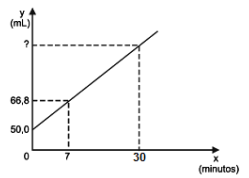
\includegraphics[scale=0.8]{figures/q10.png}
\end{Figure}
\begin{enumerate}[label=\alph*)]
	\item Qual a função que relaciona a quantidade \textit{y}, em \textit{ml} com o tempo \textit{x}, em minutos? 
	\item Qual a quantidade \textit{y}, em \textit{ml}, acumulada após $30$ minutos?
\end{enumerate}

\ex{16} Considere o gráfico a seguir de uma função real afim $f(x)$.
\begin{Figure}
 \centering
 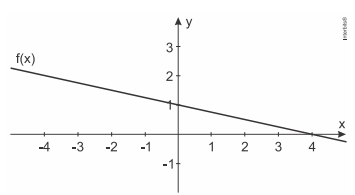
\includegraphics[scale=0.7]{figures/q11.png}
\end{Figure}
A função afim $f(x)$ é dada por:
\begin{enumerate}[label=\alph*)]
	\item $f(x) = -4x+1$
	\item $f(x) = -0.25x+1$
	\item $f(x) = -4x+4$
	\item $f(x) = -0.25x-3$
	\item $f(x) = -0.4x+1$
\end{enumerate}

\ex{17} O gráfico abaixo representa o consumo de bateria de um celular entre as $10h$ e as $16h$ de um determinado dia.
\begin{Figure}
	\centering
	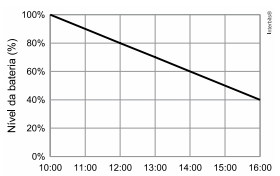
\includegraphics[scale=0.7]{figures/q12.png}
\end{Figure}
Supondo que o consumo manteve o mesmo padrão até a bateria se esgotar, a que horas o nível da bateria atingiu $10\%$?

\begin{enumerate}[label=\alph*)]
	\item $18h$
	\item $19h$
	\item $20h$
	\item $21h$
	\item $22h$
\end{enumerate}

\end{multicols}

%----------------------Gabarito---------------------------------------------
\newpage
\begin{multicols}{2}
[
\begin{center}
\section*{Gabarito}
\end{center}
]

\end{multicols}
\end{document}
